\section{Week 5-6}
\subsection{Objective}
For the final section of the project, we will try to see how to combine the Bayesian Optimal Design problem from week 2 with the variational inference framework from week 3-4, 
leading to a general framework for Bayesian Optimal Design that scales to many different kinds of model.
% The objective of this week is to integrate our Bayesian Optimal Design optimizer from week 2 with our linear regression variational inference optimizer from week 3.
\subsection{Theory}
\subsubsection{Finding the Gradient of the Mutual Information}
In week 2, we neatly assumed that \texttt{autograd.grad} was able to find the gradient 
of the mutual information with respect to $\B{d}$. 
When one uses variational inference to compute the posterior, this becomes nontrivial, since one needs to differentiate through the parameters as a function of the design $\B{d}$ \cite{lorraine19}.
We can see this from \eqref{eq:mi}:
\begin{equation}I(\B{d}) = \mathbb{E}_{\B{\theta}}[\mathbb{E}_{\B{y} | \theta, \B{d}}[\log (p(\theta | \B{y}, \B{d})) - \log p(\theta)]]\end{equation}
When using variational inference, this changes to
\begin{equation}\label{eq:variational-mi}I(\B{d}) \approx \mathbb{E}_{\B{\theta}}[\mathbb{E}_{\B{y}|\theta, \B{d}}[\log (q^*(\theta)) - \log p(\theta)]],\ \textrm{where}\ q^*(\theta) = \arg \max_q \textsc{ELBO}_{\B{d}, \B{y}}(q)\end{equation}
From now on, we will explicitly denote what $\B{d}$ and $\B{y}$ the ELBO is taken with regards to.
Taking the gradient of \eqref{eq:variational-mi} and using reparamerization results in
\begin{equation}\nabla_\B{d} I(\B{d}) = \nabla_\B{d}\mathbb{E}_{\B{\theta}}[\mathbb{E}_{\B{y} | \theta, \B{d}}[\log (q^*(\theta)) - \log p(\theta)]]\label{eq:var-mi-reparam}\end{equation}
\begin{equation} \approx \mathbb{E}_{\B{z}}[\mathbb{E}_{\B{\epsilon}}[\nabla_\B{d}\log (q^*_{\B{y}', \B{d}}(\theta'))]],\label{eq:inner-grad}\end{equation}
$$\ \textrm{where}\ \B{y}' = \B{d}\theta' + \epsilon,\ \theta' = \mu_\theta + \B{A}_\theta\B{z},\ \epsilon \sim \mathcal{N}(0, \sigma^2_\B{y} I_N),\ \B{z} \sim \mathcal{N}(0, I_M)$$
Using the chain rule gives us
\begin{equation}
  = \mathbb{E}_{\B{z}}[\mathbb{E}_{\B{\epsilon}}[\frac{1}{q^*_{\B{y}', \B{d}}(\theta')} \times \nabla_\B{d} q^*_{\B{y}', \B{d}}(\theta'))]],
  \label{eq:variational-mi-2}
\end{equation}
Thus we need to calculate $\nabla_\B{d} q^*_{\B{y}', \B{d}}(\theta')$, or more specifically
\begin{equation}
\nabla_\B{d} q^*_{\B{y}', \B{d}}(\theta') = \nabla_\B{d} \arg \max_q \textsc{ELBO}_{\B{d}, \B{y}'}(q)\Bigr\rvert_{\theta}
\end{equation}
If we let $\lambda$ be the parameters of $q$ encoded as a vector, we can regard $q^*$ as a function of $\B{d}$.
Thus we can use the chain rule.
\begin{equation}
  \nabla_\B{d} q^*_{\B{y}', \B{d}}(\theta') = \nabla_\lambda q^{\lambda}_{\B{y}', \B{d}}(\theta')\underbrace{\nabla_\B{d} \arg \max_\lambda \textsc{ELBO}_{\B{d}, \B{y}'}(q^\lambda)}_{\textrm{Jacobian}}
\end{equation}
The gradient, $\nabla_\lambda q^\lambda_{\B{y}',\B{d}}$, is simple to perform using automatic differentiation.
The Jacobian of the variational parameters with regards to the design $\B{d}$, needs very careful consideration. 
We will approach this using the Implicit Function Theorem \cite{lorraine19}:
\begin{theorem}
  Let $f$ be a continuously differentiable function from $\mathbb{R}^n \times \mathbb{R}^m$ to $\mathbb{R}^m$.
  Fix a point $(a, b)$ such that $f(a, b) = \B{0}$. 
  If the Jacobian $J_b^{f}(a, b)$ is invertible, then there must exist an open set $U \subseteq \mathbb{R}^n$ containing $a$
  such that there exists a continuously differentiable function $g: U \rightarrow \mathbb{R}^m$ such that $g(a) = b$ and $f(x, g(x)) = \B{0}$ for all $x \in U$.
  Furthermore,
  $$\nabla_{x}g(x) = -[J_y^f(x, g(x))]^{-1}J_{x}^{f}(x, g(x))$$
  \label{thm:ift}
\end{theorem}
We will now adapt Theorem \ref{thm:ift} to our problem. 
From now on, every mention of ELBO is with regards to $\B{y} = \theta \B{d} + \epsilon$ from \eqref{eq:var-mi-reparam} .
Let $x=\B{d}$, $y=\lambda$, $g(\B{d}) = \arg \max_{\lambda} \textsc{ELBO}_{\B{d}}(q^{\lambda})$, $f(\B{d}, \lambda) = \nabla_{\lambda}\textsc{ELBO}_{\B{d}}(q^{\lambda})$.
\\
First, we need to fix a point $(\B{d}', \lambda')$ such that $\nabla_{\lambda}\textsc{ELBO}_{\B{d}'}(q^{\lambda'}) = 0$.
If we take any $\B{d}'$, and pick $\lambda'$ to be any local optimum $\lambda' = g(\B{d'})$, then the gradient must be $0$ at that point.
If the hessian then is invertible, we must have:
\begin{equation}
  \nabla_{\B{d}} \arg \max_{\lambda} \textsc{ELBO}_{\B{d}}(q^{\lambda})\Bigr\rvert_{\theta}= 
  -[\underbrace{\nabla^2_{\lambda} \textsc{ELBO}_{\B{d}}(q^*)}_{\textrm{variational hessian}}]^{-1}
  \underbrace{\nabla_{\lambda}\nabla_{\B{d}}\textsc{ELBO}_{\B{d}}(q^*)}_{\textrm{variational mixed partials}}
  \label{eq:variational-jacobian}
\end{equation}
Computing both the variational hessian and the variational mixed partials should then be possible using automatic differentiation.
\subsubsection{Adapting to Sampling}
Again, we will approach calculating the expectations using Monte Carlo sampling. From \eqref{eq:variational-mi-2}, we will instead compute
\begin{equation}\nabla_\B{d} I(\B{d}) \approx \sum_{i}^N \sum_{j}^M \frac{1}{q^*_{\B{d}, \B{y}_{ij}}(\theta_{j})}\times \nabla_{\B{d}}q^*_{\B{d}, \B{y}_{ij}}(\theta_{j})\end{equation}
$$\ \textrm{where}\ \B{y}_{ij} = \B{d}\theta_j + \epsilon_i,\ \theta_j = \mu_\theta + \B{A}_\theta\B{z}_j,\ \epsilon_i \sim \mathcal{N}(0, \sigma^2_\B{y} I_\ell),\ \B{z} \sim \mathcal{N}(0, I_M)$$

\subsection{Implementation}
\subsubsection{Reducing Computation Time}
Since both the Mutual Information gradient and variational inference algorithm utilize sampling, a naive implementation could easily end up with many nested for-loops.
To reduce this, batching techniques can be used to delegate computation to \texttt{numpy}, which can perform them in a lower level language. 
A big bottleneck is the computation of the Hessian and Jacobian of \eqref{eq:variational-jacobian}, which can be sped up by using more modern automatic differentiation libraries than \texttt{autograd}.
\subsubsection{Correctness of Implementation}
Since we have the code and theoretical knowledge for each of the components that this implementation is composed of, 
we can test each part of the implementation by comparing it to its analytical counterpart. 
For example, one can replace the variational approximation with the analytical posterior to see how the variational approximation change the convergence of the Mutual Information metric.
One can furthermore compare this to the results from week 2, where we used automatic differentiation to compute the entire gradient of the Mutual Information metric.
\subsection{Results}
It was not possible within the scope of this project to get a fully working implementation of the combined Bayesian Optimal Design and variational inference algorithms.
One of the main problems is that a lot of noise is introduced when we compute the gradient ourselves. 
The following code snippet uses autograd to compute the gradient inside the expectations of \eqref{eq:inner-grad}:
\begin{minted}{python}
def MI_grad(d):
    N = 5
    M = 1
    results = []
    eps = np.random.randn(N, len(d)) * np.sqrt(noise)
    for i in range(N):
        zs = np.random.randn(M, 3)
        for j in range(M):
            theta_j = mu_prior + A_prior @ zs[j]
            y_ij = augment_d(d) @ theta_j + eps[i]
            def g(d):
                mean, cov = analytical_posterior_params(augment_d(d), y_ij, mu_prior=mu_prior, cov_prior=cov_prior)
                return mean, np.linalg.cholesky(cov)
            def q_(theta, lam):
                mean, A = lam
                return stable_multivariate_gaussian_logpdf(theta, mean, A @ A.T)
            results.append(encode_d(grad(lambda d: q_(theta_j, g(d)))(d)))
    return decode_d(np.mean(np.array(results), axis=0), dim=2)
\end{minted}
This code produces results that can be shown in Figure \ref{fig:mi-1-var}. 
As it can be seen, while it seems like the Mutual Information is very slowly rising, the algorithm is much more noisy, 
and does not produce plots that look like the ones we saw in week 2 - even when the two implementations should be equivalent.\\
\begin{figure}
  \centering
  \begin{subfigure}{0.45\textwidth}
    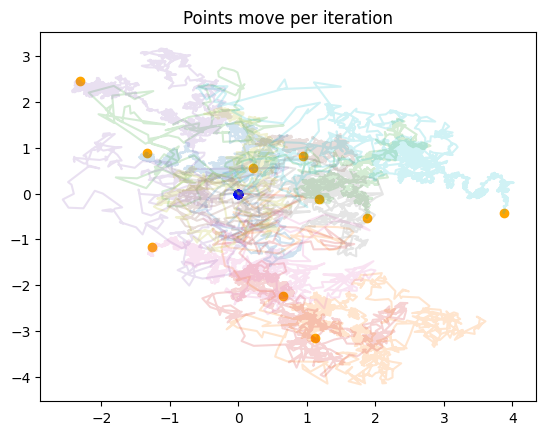
\includegraphics[width=\linewidth]{week4/mi-1-many.png}
  \end{subfigure}
  \begin{subfigure}{0.45\textwidth}
    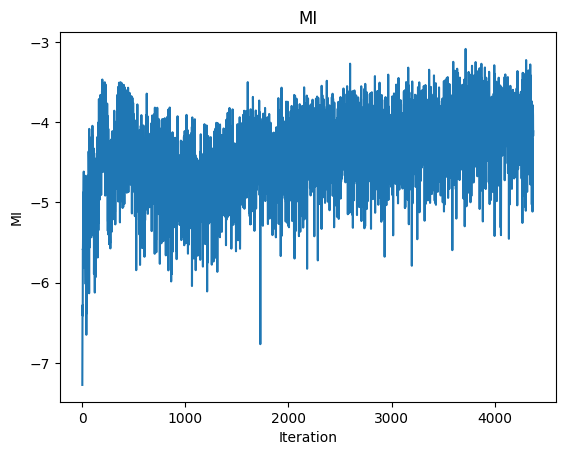
\includegraphics[width=\linewidth]{week4/mi-1-after-many.png}
  \end{subfigure}
  \caption{Movement of points using gradient from \eqref{eq:var-mi-reparam}. Blue is start position, orange is end position.}
  \label{fig:mi-1-var}
\end{figure}
If this did work, we could implement the entire gradient of the Mutual Information like so.
\begin{minted}{python}
def q_grad(theta, q_params, d, y_i):
    q_mean, q_A = q_params
    inverse_hessian = np.linalg.inv(hessian(lambda eq: ELBO(augment_d(d), y_i, decode_q_params(eq)[0], decode_q_params(eq)[1]))(encode_q_params(q_params)))
    mixed_partials = jacobian(lambda eq: grad(lambda d: ELBO(augment_d(decode_d(d, dim=2)), y_i, decode_q_params(eq)[0], decode_q_params(eq)[1]))(encode_d(d)))(encode_q_params(q_params)).T
    jac = - inverse_hessian @ mixed_partials
    return jac
def MI_grad_5(d):
    N = 5
    M = 1
    results = []
    eps = np.random.randn(N, len(d)) * np.sqrt(noise)
    for i in range(N):
        zs = np.random.randn(M, 3)
        for j in range(M):
            theta_j = mu_prior + A_prior @ zs[j]
            y_ij = augment_d(d) @ theta_j + eps[i]
            def g(d):
                mean, cov = analytical_posterior_params(augment_d(d), y_ij, mu_prior=mu_prior, cov_prior=cov_prior)
                return mean, np.linalg.cholesky(cov)
            def q_(theta, lam):
                mean, A = lam
                return stable_multivariate_gaussian_logpdf(theta, mean, A @ A.T)
            
            def inner_objective_f(encoded_q_params):
                mean, A = decode_q_params(encoded_q_params)
                elbo = ELBO(augment_d(d), y_ij, mean, A)
                return -elbo
            q_params = decode_q_params(optimize(grad(inner_objective_f), encode_q_params((mu_prior, A_prior)), 1e-1, 2, 0, 1e2))
            g1 = encode_q_params(grad(lambda lam: q_(theta_j, lam))(q_params))
            g2 = q_grad(theta_j, q_params, d, y_ij)
            actual = g1 @ g2
            c_part = 1/q_(theta_j, q_params)
            results.append(c_part * actual)
    return np.mean(np.array(results), axis=0)
\end{minted}
Running the nested optimization is very inefficient, with one iteration of the outer optimization algorithm taking $\sim 29$ seconds on an average laptop.
Testing shows that if one replaces the inner optimization result (\texttt{q\_params}) with one obtained through the analytical posterior, the results are similar to that of Figure \ref{fig:mi-1-var}.
If one instead uses the variational posterior, the gradient becomes very large and thus the components of \textbf{d} quickly become too large to represent using floating point numbers. 
Reducing the learning rate by a factor of $10^{-2}$ can mitigate this partially
but the points still behave very erratically. An example of this can be seen in Figure \ref{fig:mi-5-var} although this example is only after 30 iterations due to the inefficiency of the algorithm.
As it can be seen, we cannot conclude that the algorithm converges nor actively moves towards an optimum due to high noise and low amount of iterations.

\begin{figure}
  \centering
  \begin{subfigure}{0.45\textwidth}
    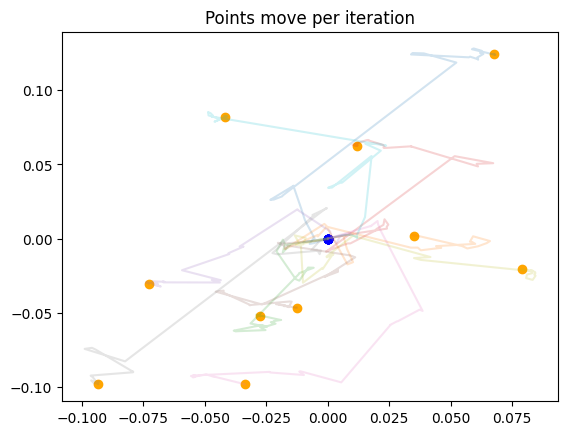
\includegraphics[width=\linewidth]{week4/mi-5-after-30-iters.png}
  \end{subfigure}
  \begin{subfigure}{0.45\textwidth}
    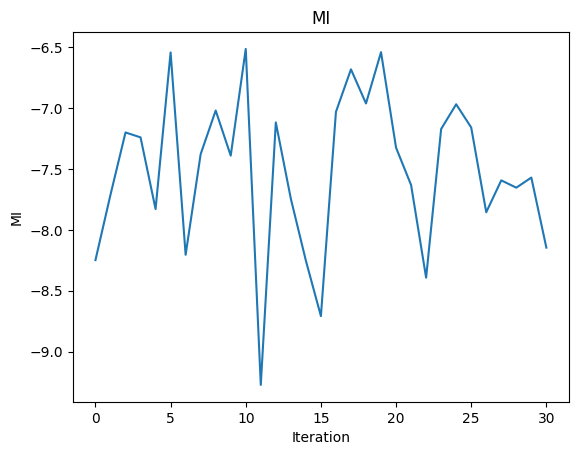
\includegraphics[width=\linewidth]{week4/mi-5-after-30-iters-plot.png}
  \end{subfigure}
  \caption{Movement of points from the full algorithm. Blue is start position, orange is end position.}
  \label{fig:mi-5-var}
\end{figure}

% \subsection{old stuff}

% \textbf{This is a working draft and should be sectioned into a more readable format, as well as have made notation consistent}
% Let us first regard our mutual information objective function from week 2:

% $$MI(\B{d})= \int_{\Theta}\int_{\B{Y}}p(\B{\theta}, \B{y}|\B{d})\log p(\B{\theta}| \B{y}, \B{d}) d\B{y}d\B{\theta}- \int_\Theta p(\theta)\log p(\B{\theta})d\B{\theta}$$
% Since we are optimizing, let us throw away the second term, since it is constant in terms of $\B{d}$:
% $$= \int_{\Theta}\int_{\B{Y}}p(\B{\theta}, \B{y}|\B{d})\log p(\B{\theta}| \B{y}, \B{d}) d\B{y}d\B{\theta}$$
% To optimize the mutual information, we will need the derivative of it in terms of $\B{d}$:
% $$\frac{\partial }{\partial \B{d}}MI(\B{d})= \frac{\partial }{\partial \B{d}}\int_{\Theta}\int_{\B{Y}}p(\B{\theta}, \B{y}|\B{d})\log p(\B{\theta}| \B{y}, \B{d}) d\B{y}d\B{\theta}$$
% $$= \int_{\Theta}\int_{\B{Y}}\frac{\partial }{\partial \B{d}}p(\B{\theta}, \B{y}|\B{d})\log p(\B{\theta}| \B{y}, \B{d}) d\B{y}d\B{\theta}$$
% Let us then use the product rule\todo{maybe change left derivative}
% $$= \int_{\Theta}\int_{\B{Y}}(\frac{\partial }{\partial \B{d}}p(\B{\theta}, \B{y}|\B{d}) \log p(\B{\theta}| \B{y}, \B{d}))
% + (p(\B{\theta}, \B{y}|\B{d})\frac{\partial }{\partial \B{d}}\log p(\B{\theta}| \B{y}, \B{d}))
%  d\B{y}d\B{\theta}$$
%  Now, let us use the fact that $\frac{\partial }{\partial \B{d}}p(\B{\theta}, \B{y}|\B{d}) = p(\theta, \B{y}|\B{d})\frac{\partial }{\partial \B{d}}\log p(\theta |\B{y}, \B{d})$ \todo{prove this lemma}
% $$= \int_{\Theta}\int_{\B{Y}}p(\theta, \B{y}|\B{d})\frac{\partial }{\partial \B{d}}\log p(\theta |\B{y}, \B{d})\log p(\theta |\B{y}, \B{d})
% + p(\B{\theta}, \B{y}|\B{d})\frac{\partial }{\partial \B{d}}\log p(\B{\theta}| \B{y}, \B{d})
%  d\B{y}d\B{\theta}$$
% $$= \int_{\Theta}\int_{\B{Y}}p(\theta, \B{y}|\B{d})\frac{\partial }{\partial \B{d}}\log p(\theta |\B{y}, \B{d})(\log p(\theta |\B{y}, \B{d}) + 1)
%  d\B{y}d\B{\theta}$$
% $$= \int_{\Theta}\int_{\B{Y}}p(\B{y}|\theta, \B{d})p(\theta)\frac{\partial }{\partial \B{d}}\log p(\theta |\B{y}, \B{d})(\log p(\theta |\B{y}, \B{d}) + 1)
%  d\B{y}d\B{\theta}$$
%  Solving this double integral can be hard. Let us consider it as an expectation of the form
%  $$\mathbb{E}[f(\theta, \B{y})]=\int_{(\theta, \B{y})} p(\theta, \B{y})f(\theta, \B{y})d(\theta, \B{y})$$
%  with $p(x)=p(\B{y}|\theta, \B{d})p(\theta)$ and $f(x)=\frac{\partial }{\partial \B{d}}\log p(\theta |\B{y}, \B{d})(\log p(\theta |\B{y}, \B{d}) + 1)$.
%  We can then approximate this expectation by sampling by reducing the expectation to:
%  $$\mathbb{E}[f(x)]\approx \frac{1}{N}\sum_{i=0}^Nf(\theta_i, \B{y}_i),\quad (\theta_i, \B{y}_i)\sim p(\theta_i, \B{y}_i)$$\todo{Figure out specific notation here}
%  which leads to
% %  We can try to approximate the outer integral by sampling: picking a set of $\theta$'s and then averaging the result of these.
% % Each $\B{y}$ can then be seen as a function of $\B{d}$ and $\theta_i$ of the form $\B{y}=\theta_i^T\B{d} + \epsilon$ where $\epsilon \sim \mathcal{N}(0, \sigma^2_\B{y})$.
% % Thus, we can also approximate the inner integral by sampling $\epsilon$ from $\mathcal{N}(0, \sigma^2_\B{y})$. Thus we get the form\todo{remove two first terms}
%  $$\frac{\partial}{\partial\B{d}}MI(\B{d})= \frac{1}{N}\sum_{i=1}^N\frac{\partial }{\partial \B{d}}\log p(\theta_i |\B{y}_i, \B{d})(\log p(\theta_i |\B{y}_i, \B{d}) + 1)
% $$
% where $(\theta_i, \B{y}_i)\sim p(\B{y}_i|\theta_i, \B{d})p(\theta_i)$.
% Sampling $\theta_i$ is easy from our prior, and we can do reparameterization to sample $\B{y}_{ij}=\theta_i^T \B{d} + z_j$ where $z_j\sim \mathcal{N}(0,\sigma^2_\B{y})$.

% \subsubsection{Finding the gradient of the posterior}
% \textbf{Notation}:\\
% $\vartheta$ = $\mu_\theta$ and $A_\theta$ for use in $q_{\vartheta}$\\
% $\B{y}_\B{d}$ = $\B{y}$ calculated from $\B{d}$.\\
% Now, let us consider the posterior $p(\theta_i|\B{y}, \B{d})$. This is the distribution that we try to approximate when performing variational inference. 
% Thus we can expect our variational distribution $q(\theta_i)$ to reasonably approximate it after our inference algorithm has run.
% We will denote the optimal parameters found $\vartheta^*(\B{d}, \B{y}_\B{d}) = \arg \max_\vartheta \textsc{ELBO}_{\B{d}, \B{y}(\B{d})}(q_\vartheta)$ such that $q_{\vartheta^*}(\theta_i)\approx p(\theta_i | \B{y}_\B{d}, \B{d})$.\\
% In our refactored expression for mutual information, we have a term containing $\frac{\partial }{\partial \B{d}}\log p(\theta_i |\B{y}_\B{d}, \B{d})$.

% % Thus, we can regard $\frac{\partial }{\partial \B{d}}\log p(\theta_i|\B{y}, \B{d})$ as
% % the derivative (in regards to $\B{d}$) of our variational distribution, evaluated at some point $\theta_i^*$(\B{y}, \B{d}) (which is the best possible configuration of parameters given $\B{y}$ and $\B{d}$).\\
% % Being that our 
% % Our inference algorithm takes $\B{y}$ and $\B{d}$ as input as well, which we will call $\B{w}$.
% % Evaluating $\frac{\partial }{\partial \B{d}}\log p(\theta_i|\B{y}, \B{d})$ can thus take the form:
% % $$\frac{\partial }{\partial \B{d}}\log p(\theta_i|\B{y}, \B{d}) = \frac{\partial }{\partial \B{d}}\log q(\theta_i)\Bigr\rvert_{\theta_i = \theta_i^*(\B{y}, \B{d})}$$
% $$\frac{\partial }{\partial \B{d}}\log p(\theta_i|\B{y}_\B{d}, \B{d}) \approx \frac{\partial }{\partial \B{d}}\log q_{\vartheta^*}(\theta_i)$$
% Since $\vartheta^*$ is a function of $\B{d}$, and $q^*$ is a function of $\theta^*$, then we can use the chain rule.
% $$=\frac{\partial}{\partial \vartheta^*}\log q_{\vartheta^*}(\theta_i)\frac{\partial }{\partial \B{d}}\vartheta^*(\B{y}_\B{d}, \B{d})$$

% \subsubsection{Using The Implicit Function Theorem for finding the indirect gradient}
% Let $\mathcal{D}$ be ($\B{d}$, $\B{y}$) encoded in some vector.\\
% If for some $(\mathcal{D}', \vartheta')$, $\frac{\partial }{\partial \vartheta} \textsc{ELBO}_{\mathcal{D}'} (q_\vartheta)\Bigr\rvert_{\mathcal{D}=\mathcal{D}', \vartheta=\vartheta'} = 0$
% and the Jacobian is invertible, then there exists an open set of datapoints $\mathcal{D} \in \mathcal{X} \times \mathcal{Y}$ \todo{add reference! very similar to litterature}
% such that there exists a function $\vartheta^* \colon \mathcal{X} \times \mathcal{Y} \rightarrow \Theta $ such that
% $$\vartheta^*(\mathcal{D}')= \vartheta' \textrm{ and }\forall \mathcal{D} \in \mathcal{X}\times \mathcal{Y}, \frac{\partial }{\partial \vartheta}\textsc{ELBO}_\mathcal{D} (q_\vartheta)\Bigr\rvert_{\mathcal{D}, \vartheta^*(\mathcal{D})} = 0$$
% Another consequence of this is that we can write
% $$\frac{\partial \vartheta^*}{\partial \B{d}}\Bigr\rvert_{\B{d}'} = \left(- \left[\frac{\partial^2 \textsc{ELBO}_{\B{d}, \B{y}_i}(q_\vartheta)}{\partial \vartheta \partial \vartheta^T}\right]^{-1}\times \frac{\partial^2 \textsc{ELBO}_{\B{d}, \B{y}_i}(q_\vartheta)}{\partial \vartheta \partial \B{d}^T}\right)\Bigr\rvert_{\B{d}', \vartheta^*(\B{d}', \B{y}'_i)}$$
% Where $\B{y}_i' = \theta^T\B{d}' + \B{z}$.
% Now we have the indirect gradient.
% % $$\frac{\partial \vartheta^*}{\partial \B{d}}\Bigr\rvert_{\B{d}'} = \left(- \left[\frac{\partial^2 \textsc{ELBO}_{\B{d}, \B{y}_i}(q_\vartheta)}{\partial \vartheta \partial \vartheta^T}\right]^{-1}\times \frac{\partial^2 \textsc{ELBO}_{\B{d}, \B{y}_i}(q_\vartheta)}{\partial \vartheta \partial \B{d}^T}\right)\Bigr\rvert_{\B{d}', \vartheta^*(\B{d}', \B{y}'_i)}$$
% % $$\frac{\partial }{\partial \B{d}}\vartheta^*(\B{y}_\B{d},\B{d}) =\frac{\partial \vartheta^*}{\partial \B{w}}\Bigr\rvert_{\B{w}=(\B{y}_d,\B{d})}= \left(- \left[\frac{\partial^2 \textsc{ELBO}_\B{w}(q_\vartheta)}{\partial \vartheta \partial \vartheta^T}\right]^{-1}\times \frac{\partial^2 \textsc{ELBO}_\B{w}(q_\vartheta)}{\partial \vartheta \partial \B{w}^T}\right)\Bigr\rvert_{\B{w}=(\B{y}, \B{d}), \vartheta^*(\B{y}_d, \B{d})}$$\todo{Find where evaluation is supposed to be}
% % These two parts are especially computable using tools like Autograd.
% % From our expression of the derivative of the log-posterior, we are interested in finding 
% % We model this by multiplying the change of $\log q(\theta_i)$ by $\theta_i$ with the change of $\theta_i$ by $\B{d}$.
% % $$=\frac{\partial}{\partial \theta_i}\log q(\theta_i)\Bigr\rvert_{\theta_i = \theta_i^*(\B{y}, \B{d})}\frac{\partial}{\partial \B{d}}\theta_i^*(\B{y},\B{d})$$
% % This gives us what the litterature calls the \textit{indirect gradient} \todo{check if true, add citation}.
% % Calculating the first part of this is rather simple through automatic differentiation.
% % The second part requires a bit more carefulness, and can be achieved through using the Implicit Function Theorem:
% % If for some $(\B{d}', \theta')$, $\frac{\partial }{\partial \theta} \textsc{ELBO} (q)\Bigr\rvert_{\B{d}', \theta'} = 0$
% % and the Jacobian is invertible, then there exists an open set of datapoints $\B{d} \in \mathcal{D}$ \todo{add reference! very similar to litterature}
% % such that there exists a function $\theta^* \colon \mathcal{D} \rightarrow \Theta $ such that
% % $$\theta^*(\B{d}')= \theta' \textrm{ and }\forall \B{d} \in \mathcal{D}, \frac{\partial }{\partial \theta}\textsc{ELBO} (q)\Bigr\rvert_{\B{d}, \theta^*(\B{d})} = 0$$
% % The way to interpret this is that if there exists some optimum, then it is possible to consistently construct the parameters such that we meet this optimum.
% % In the case of variational inference, we regard our optimization procedure as an approximation of $\theta^*$.
% % A consequence of the Implicit Function Theorem is also that we can write the partial derivative of $\theta^*$ like so:
% % $$\frac{\partial \theta^*}{\partial \B{d}} = - \left[\frac{\partial^2 \textsc{ELBO}(q)}{\partial \theta \partial \theta^T}\right]^{-1}\times \frac{\partial^2 \textsc{ELBO}(q)}{\partial \theta \partial \B{d}^T}$$
% \subsection{Design}
% \subsection{Results}
% \subsection{Evalution}
